\documentclass[paper=a4, fontsize=11pt]{scrartcl} % KOMA-article class

%-------------------------------------------------
%   THEMES, PACKAGES, CUSTOM COMMANDS
%-------------------------------------------------
\usepackage{blindtext}
\usepackage[english]{babel}                             % English language/hyphenation
\usepackage[protrusion=true,expansion=true]{microtype}  % Better typography
\usepackage{amsmath,amsfonts,amsthm}                    % Math packages
\usepackage[pdftex]{graphicx}                           % Enable pdflatex
\usepackage[export]{adjustbox}
\usepackage[svgnames]{xcolor}                           % Enabling colors by their 'svgnames'
\usepackage[hang, small,labelfont=bf,up,textfont=it,up]{caption} % Custom captions under/above floats
\usepackage{subcaption}
\usepackage{epstopdf}       % Converts .eps to .pdf
%\usepackage{subfig}         % Subfigures
\usepackage{booktabs}       % Nicer tables
\usepackage{fix-cm}         % Custom fontsizes
\usepackage{listings}
\usepackage{soul}

\usepackage{hyperref}

\usepackage[foot=30pt,margin=1in]{geometry}

% Custom sectioning (sectsty package)
\usepackage{sectsty}
\allsectionsfont{
    \usefont{OT1}{phv}{b}{n}    % bch-b-n: CharterBT-Bold font
}
\sectionfont{
    \usefont{OT1}{phv}{b}{n}
}

% Custom colors
\definecolor{brsugrey}{rgb}{0.9, 0.9, 0.9}
\definecolor{brsublue}{rgb}{0, 0.594, 0.949}

%
\newcommand{\upperRomannumeral}[1]{\uppercase\expandafter{\romannumeral#1}}

% Creating an initial of the very first character of the content
\usepackage{lettrine}
\newcommand{\initial}[1]{%
    \lettrine[lines=3,lhang=0.3,nindent=0em]{
        \color{brsublue}
        {\textsf{#1}}}{}}

%-------------------------------------------------
%   COMMON INFO
%-------------------------------------------------
\newcommand{\hmwkTitle}{Week \upperRomannumeral{2} report}
\newcommand{\hmwkDueDate}{Tuesday, October 4, 2016}
\newcommand{\hmwkClass}{Scientific Evaluation and Experimentation}
\newcommand{\hmwkClassShort}{SEE WS2016}
\newcommand{\hmwkAuthorFullName}{Minh H. Nguyen \& Bach D. Ha}
\newcommand{\hmwkAuthorLastName}{Nguyen \& Ha}
\newcommand{\hmwkAuthorEmail}{minh.nguyen@smail.inf.h-brs.de\\
                              bach.ha@smail.inf.h-brs.de}
\newcommand{\hmwkAuthorInstitute}{BRS University of Applied Sciences}

%-------------------------------------------------
%   HEADERS & FOOTERS
%-------------------------------------------------
\usepackage{fancyhdr}
\pagestyle{fancy}
\usepackage{lastpage}
% Header (empty)
\lhead{}
\chead{}
\rhead{}
% Footer (you may change this to your own needs)
\lfoot{\footnotesize
    \texttt{\hmwkClassShort} ~
    \textbullet ~ \hmwkAuthorLastName ~
    \textbullet ~ \hmwkTitle}
\cfoot{}
\rfoot{\footnotesize page \thepage\ of \pageref{LastPage}}  % "Page 1 of 2"
\renewcommand{\headrulewidth}{0.0pt}
\renewcommand{\footrulewidth}{0.4pt}

%-------------------------------------------------
%   TITLE & AUTHOR
%-------------------------------------------------
\usepackage{titling}

\newcommand{\HorRule}{\color{brsublue}% Creating a horizontal rule
    \rule{\linewidth}{1pt}%
    \color{black}
}

% Title
\pretitle{
    \vspace{-30pt}
    \begin{flushleft}
        \HorRule
        \fontsize{22}{22} \usefont{OT1}{phv}{b}{n} \color{gray} \selectfont
}
\title{\hmwkClass \\
       \hmwkTitle}
\posttitle{
    \par
    \end{flushleft}
    \vskip 0.5em
}

% Author
\preauthor{
    \begin{flushleft}
        \large \lineskip 0.25em
        \usefont{OT1}{phv}{b}{sl} \color{brsublue}}

\author{\hmwkAuthorFullName}

\postauthor{
        \footnotesize
        \usefont{OT1}{phv}{m}{sl} \color{Black}
        \\\hmwkAuthorInstitute
        \\\hmwkAuthorEmail
        \par
    \end{flushleft}
    \HorRule}

% Date
\date{\hmwkDueDate}

%-------------------------------------------------
%   BEGIN
%-------------------------------------------------
\begin{document}
    \maketitle
    \thispagestyle{fancy} % Enabling the custom headers/footers for the first page

    \section{Detailed experimentation description}

    \begin{figure}[h!]
        \centering
        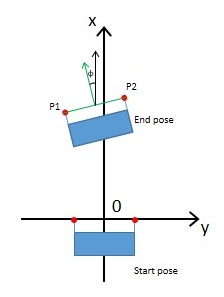
\includegraphics[width=0.6\linewidth]{images/Img1}
        \caption{Experiment setup}
        \label{fig:img1}
    \end{figure}
        
    \begin{figure}[h!]
        \centering
        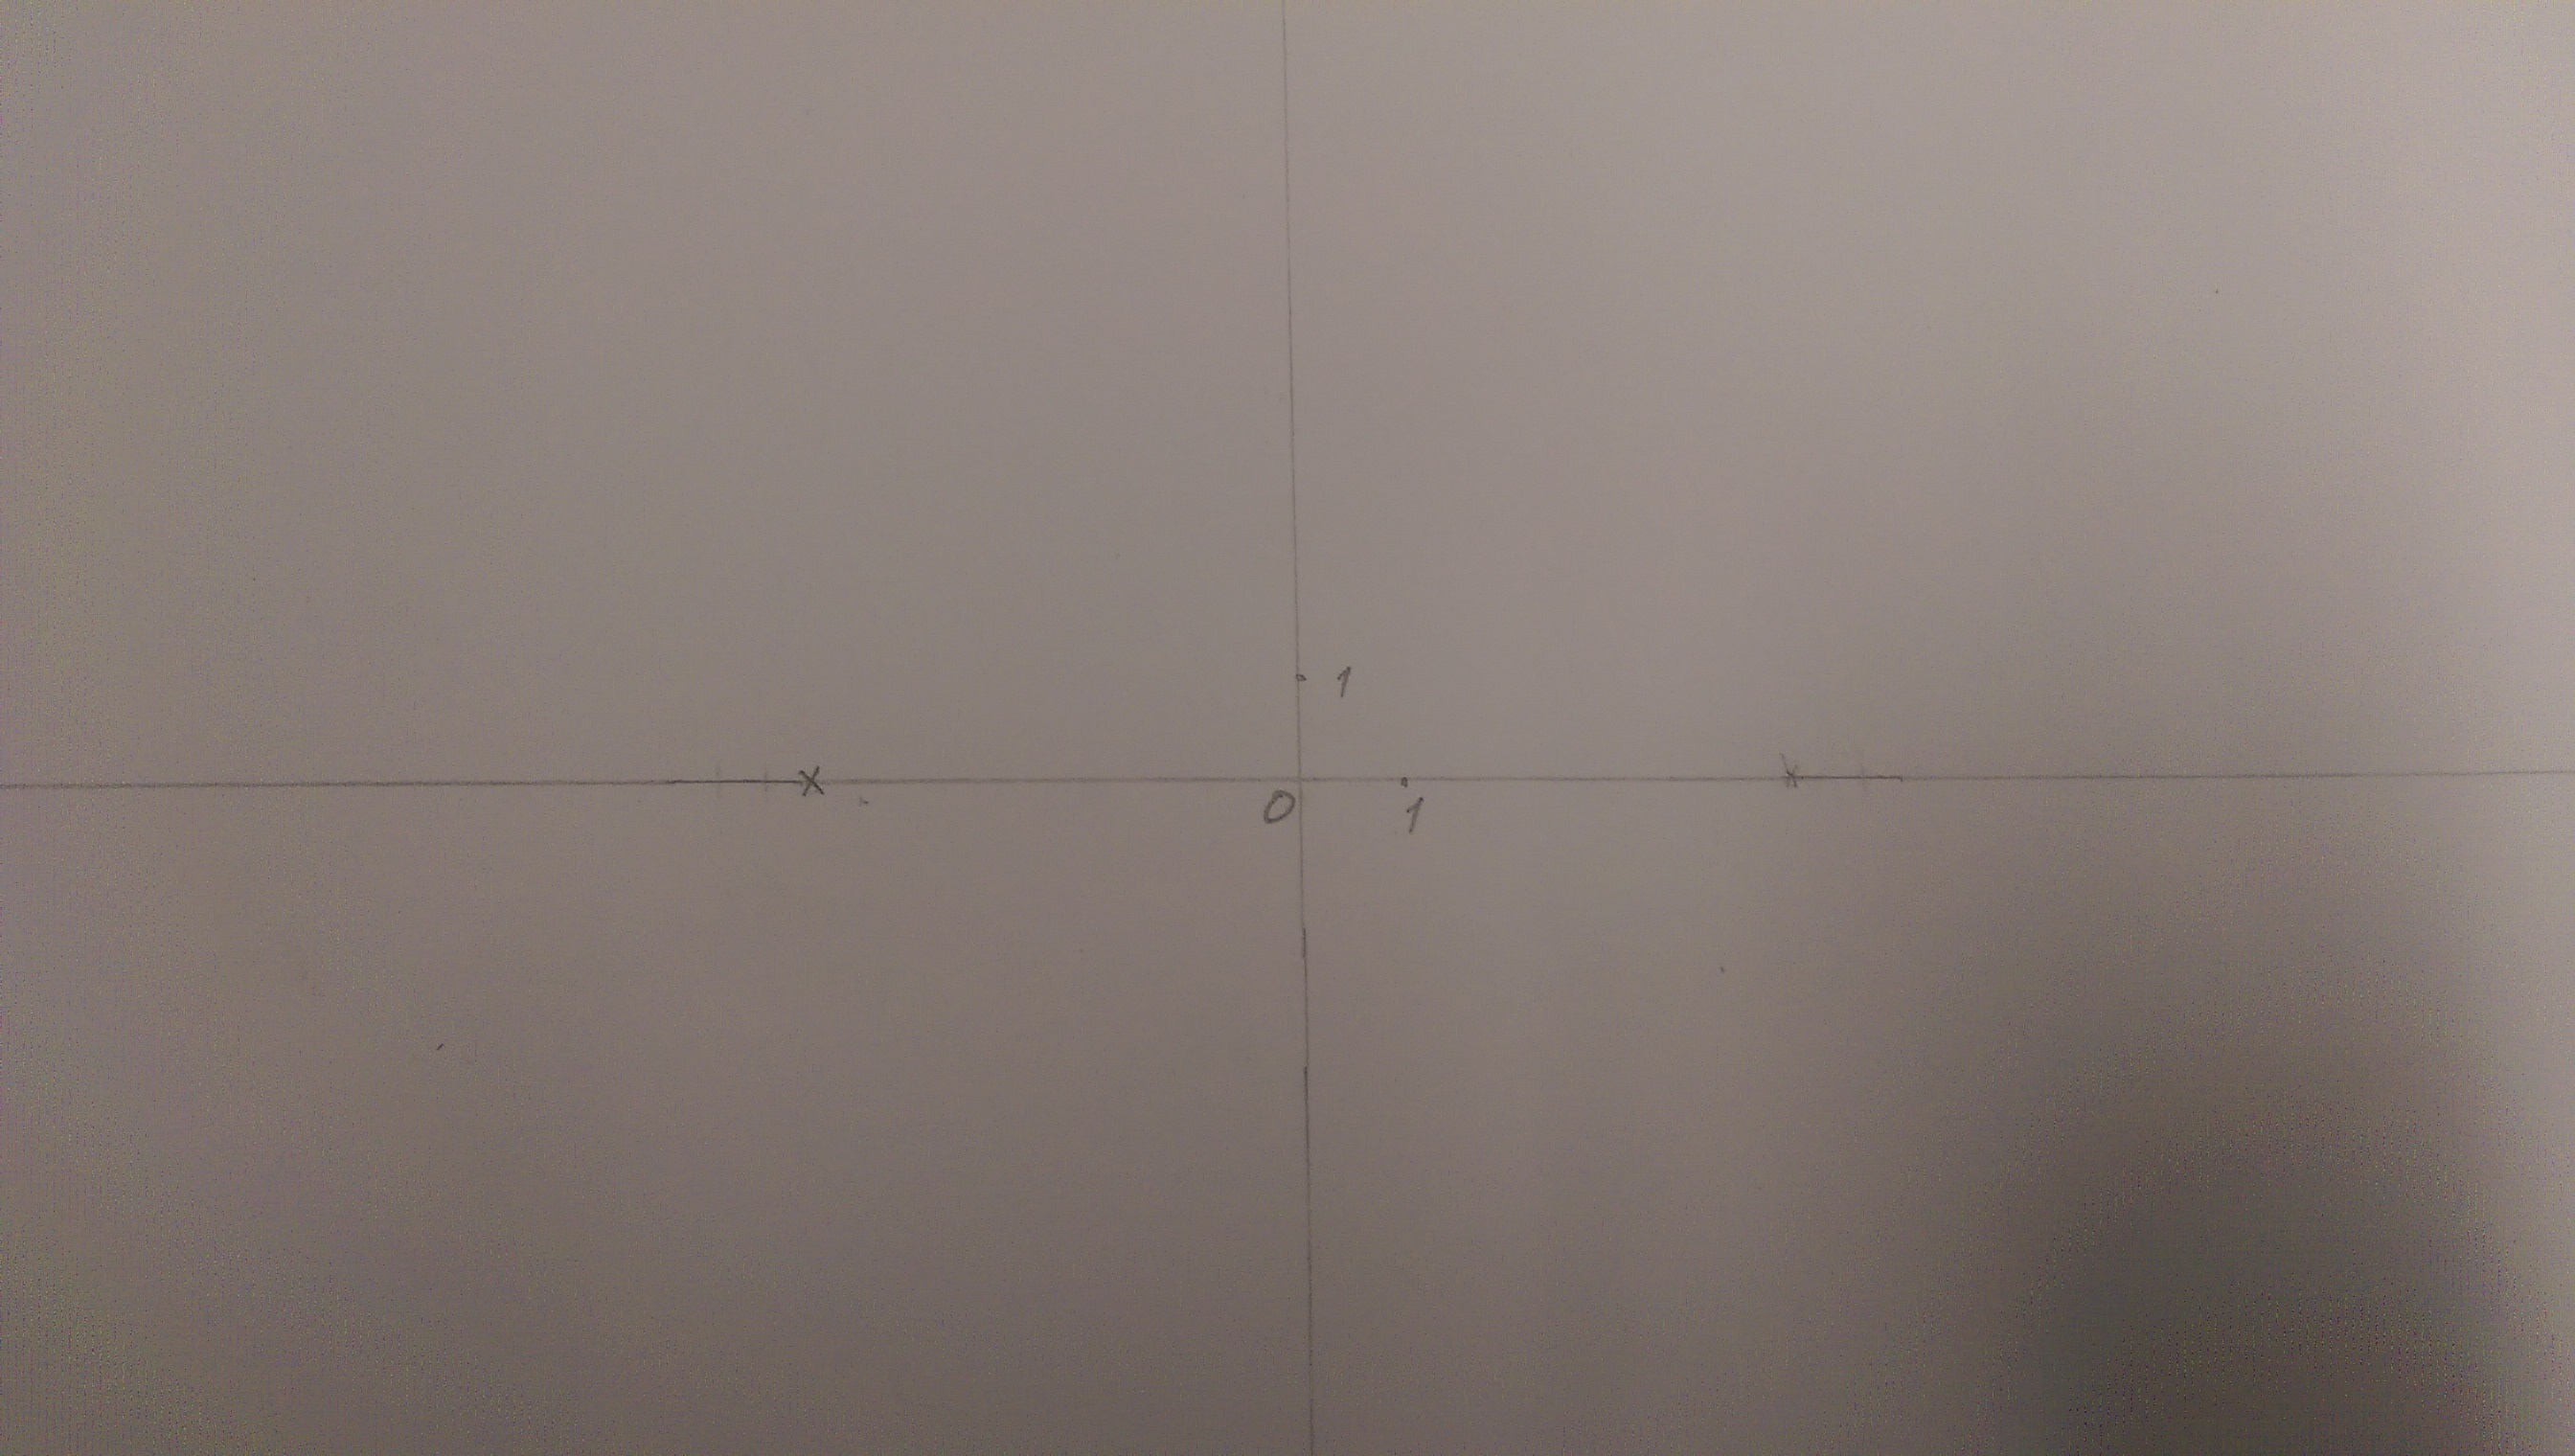
\includegraphics[width=0.9\linewidth]{images/IMAG0144}
        \caption{Starting point}
        \label{fig:img2}
    \end{figure}
    
    \begin{figure}[!tbp]
        \centering
        \begin{minipage}[b]{0.9\textwidth}
            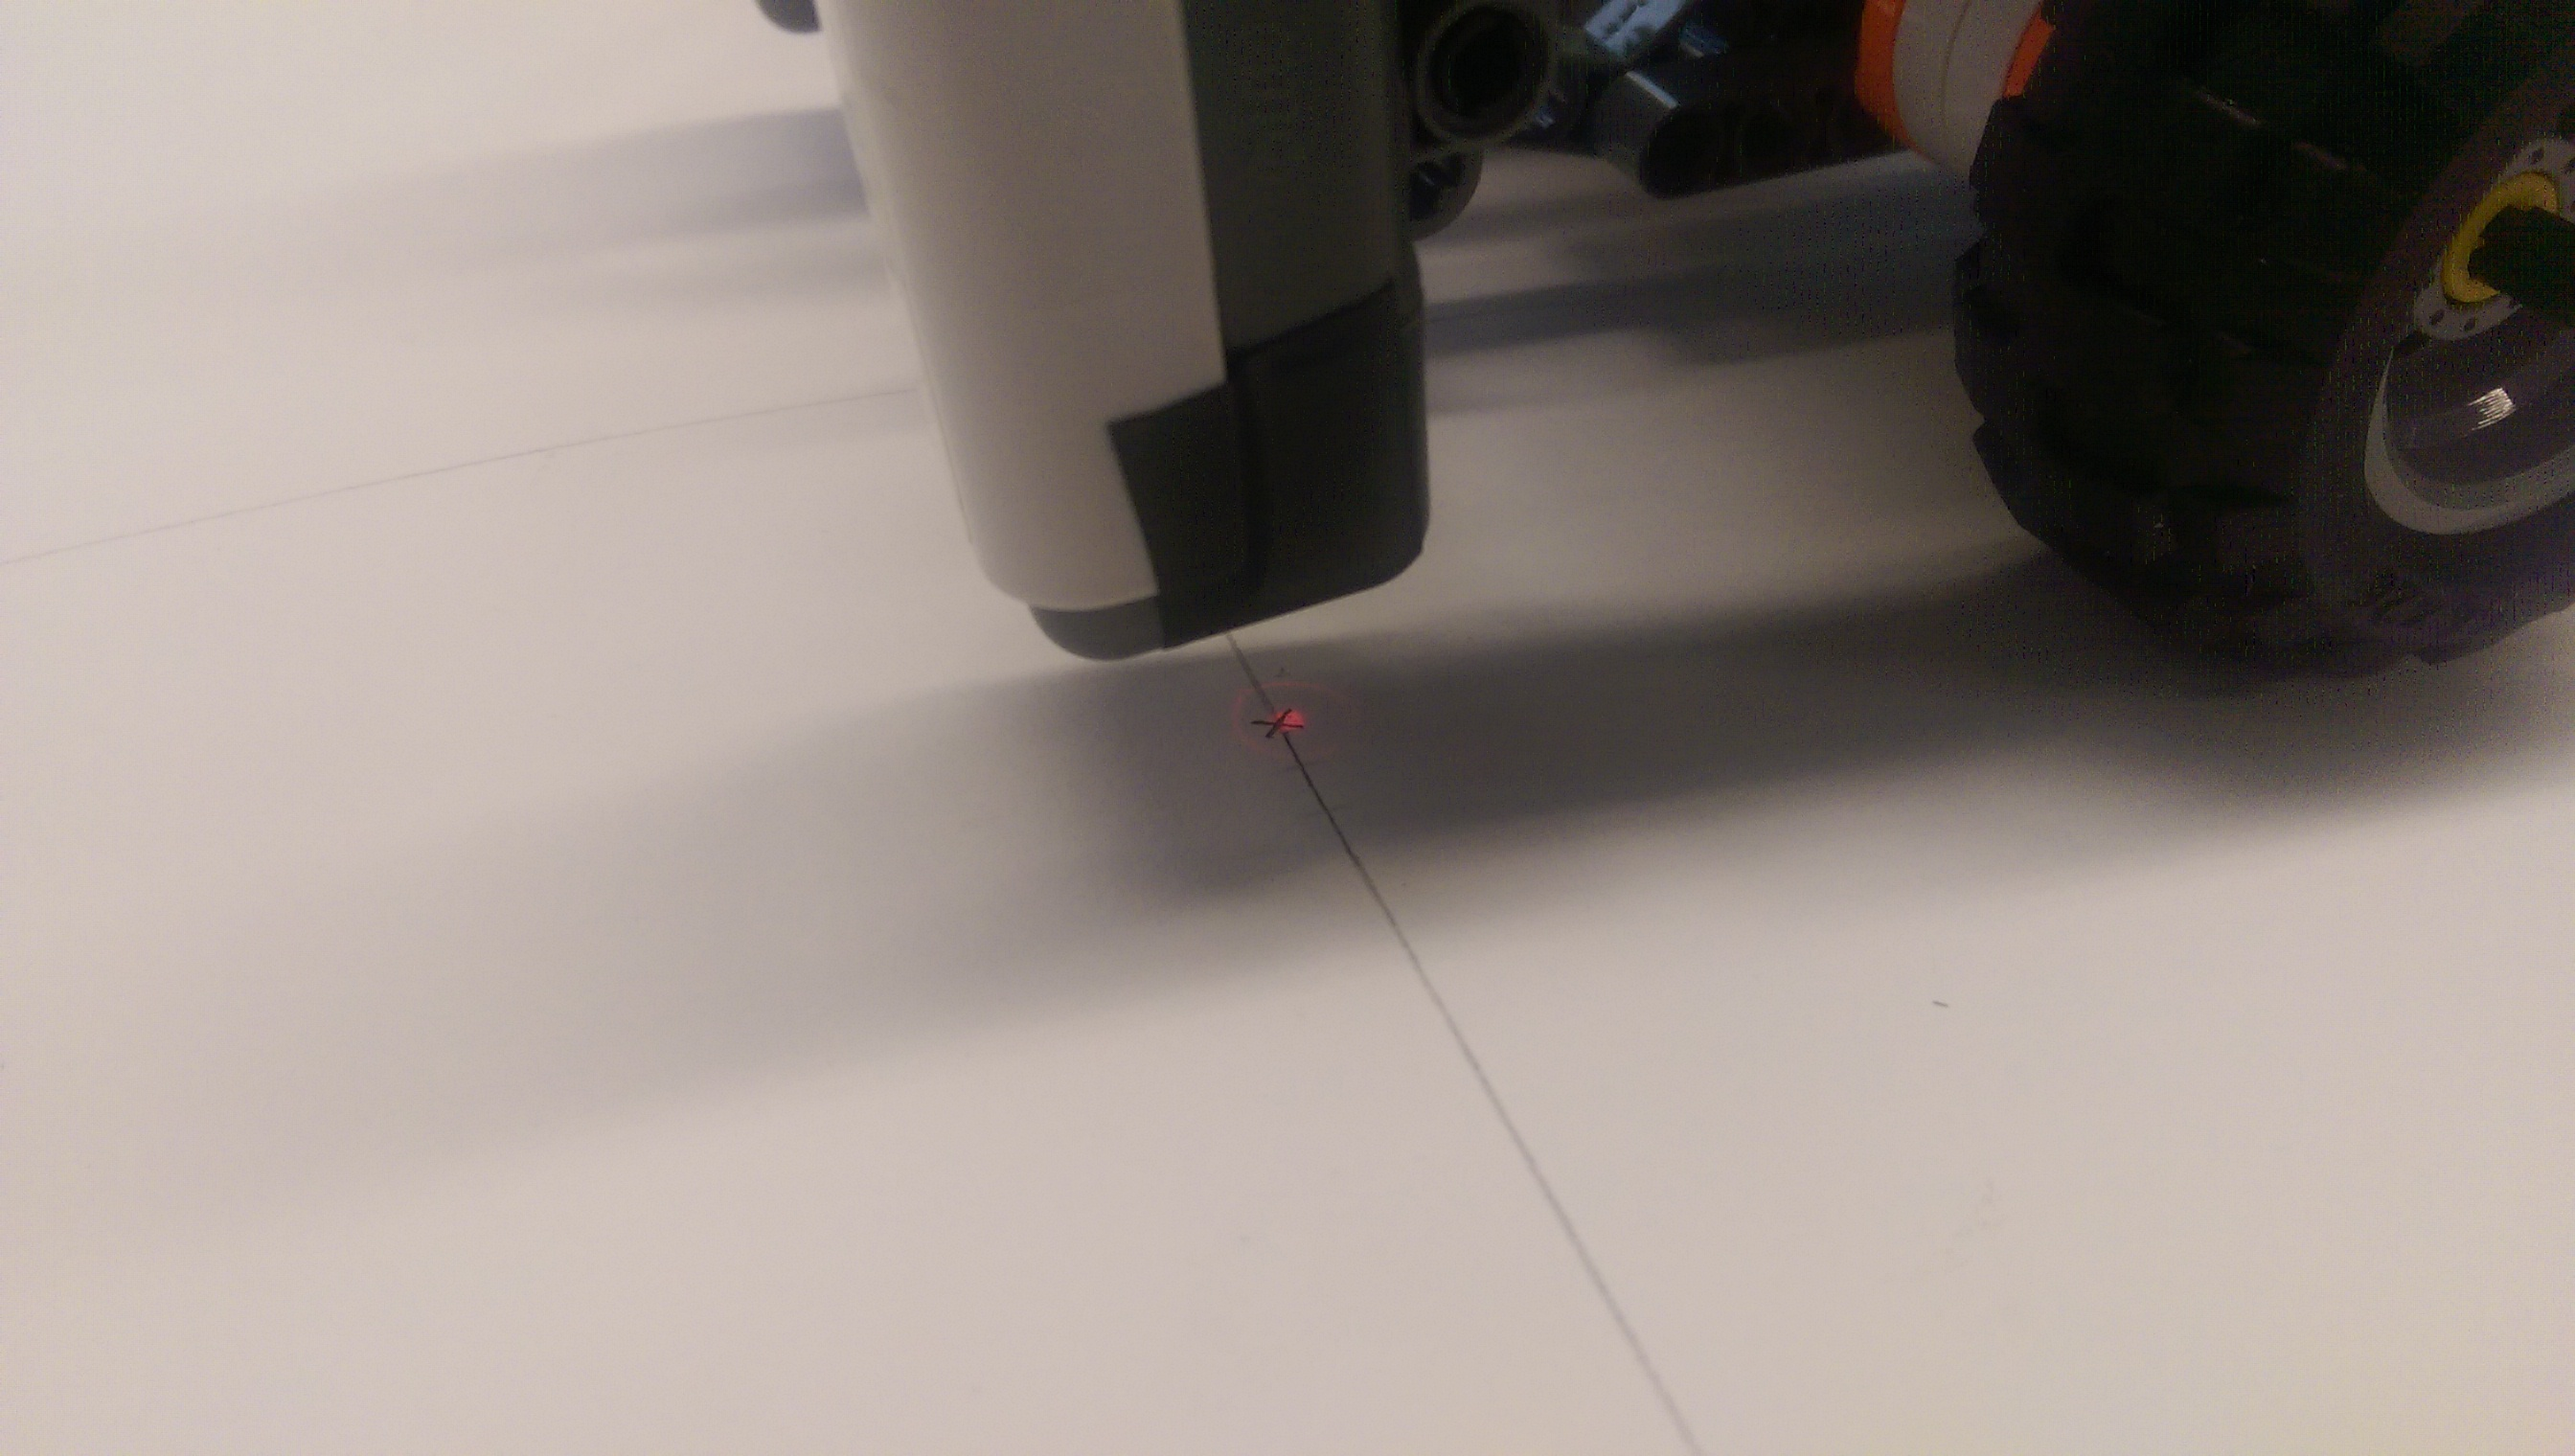
\includegraphics[width=1\linewidth]{images/IMAG0142}
            \caption{Left marker}
            \label{fig:img3}
        \end{minipage}
        \hfill
        \begin{minipage}[b]{0.9\textwidth}
            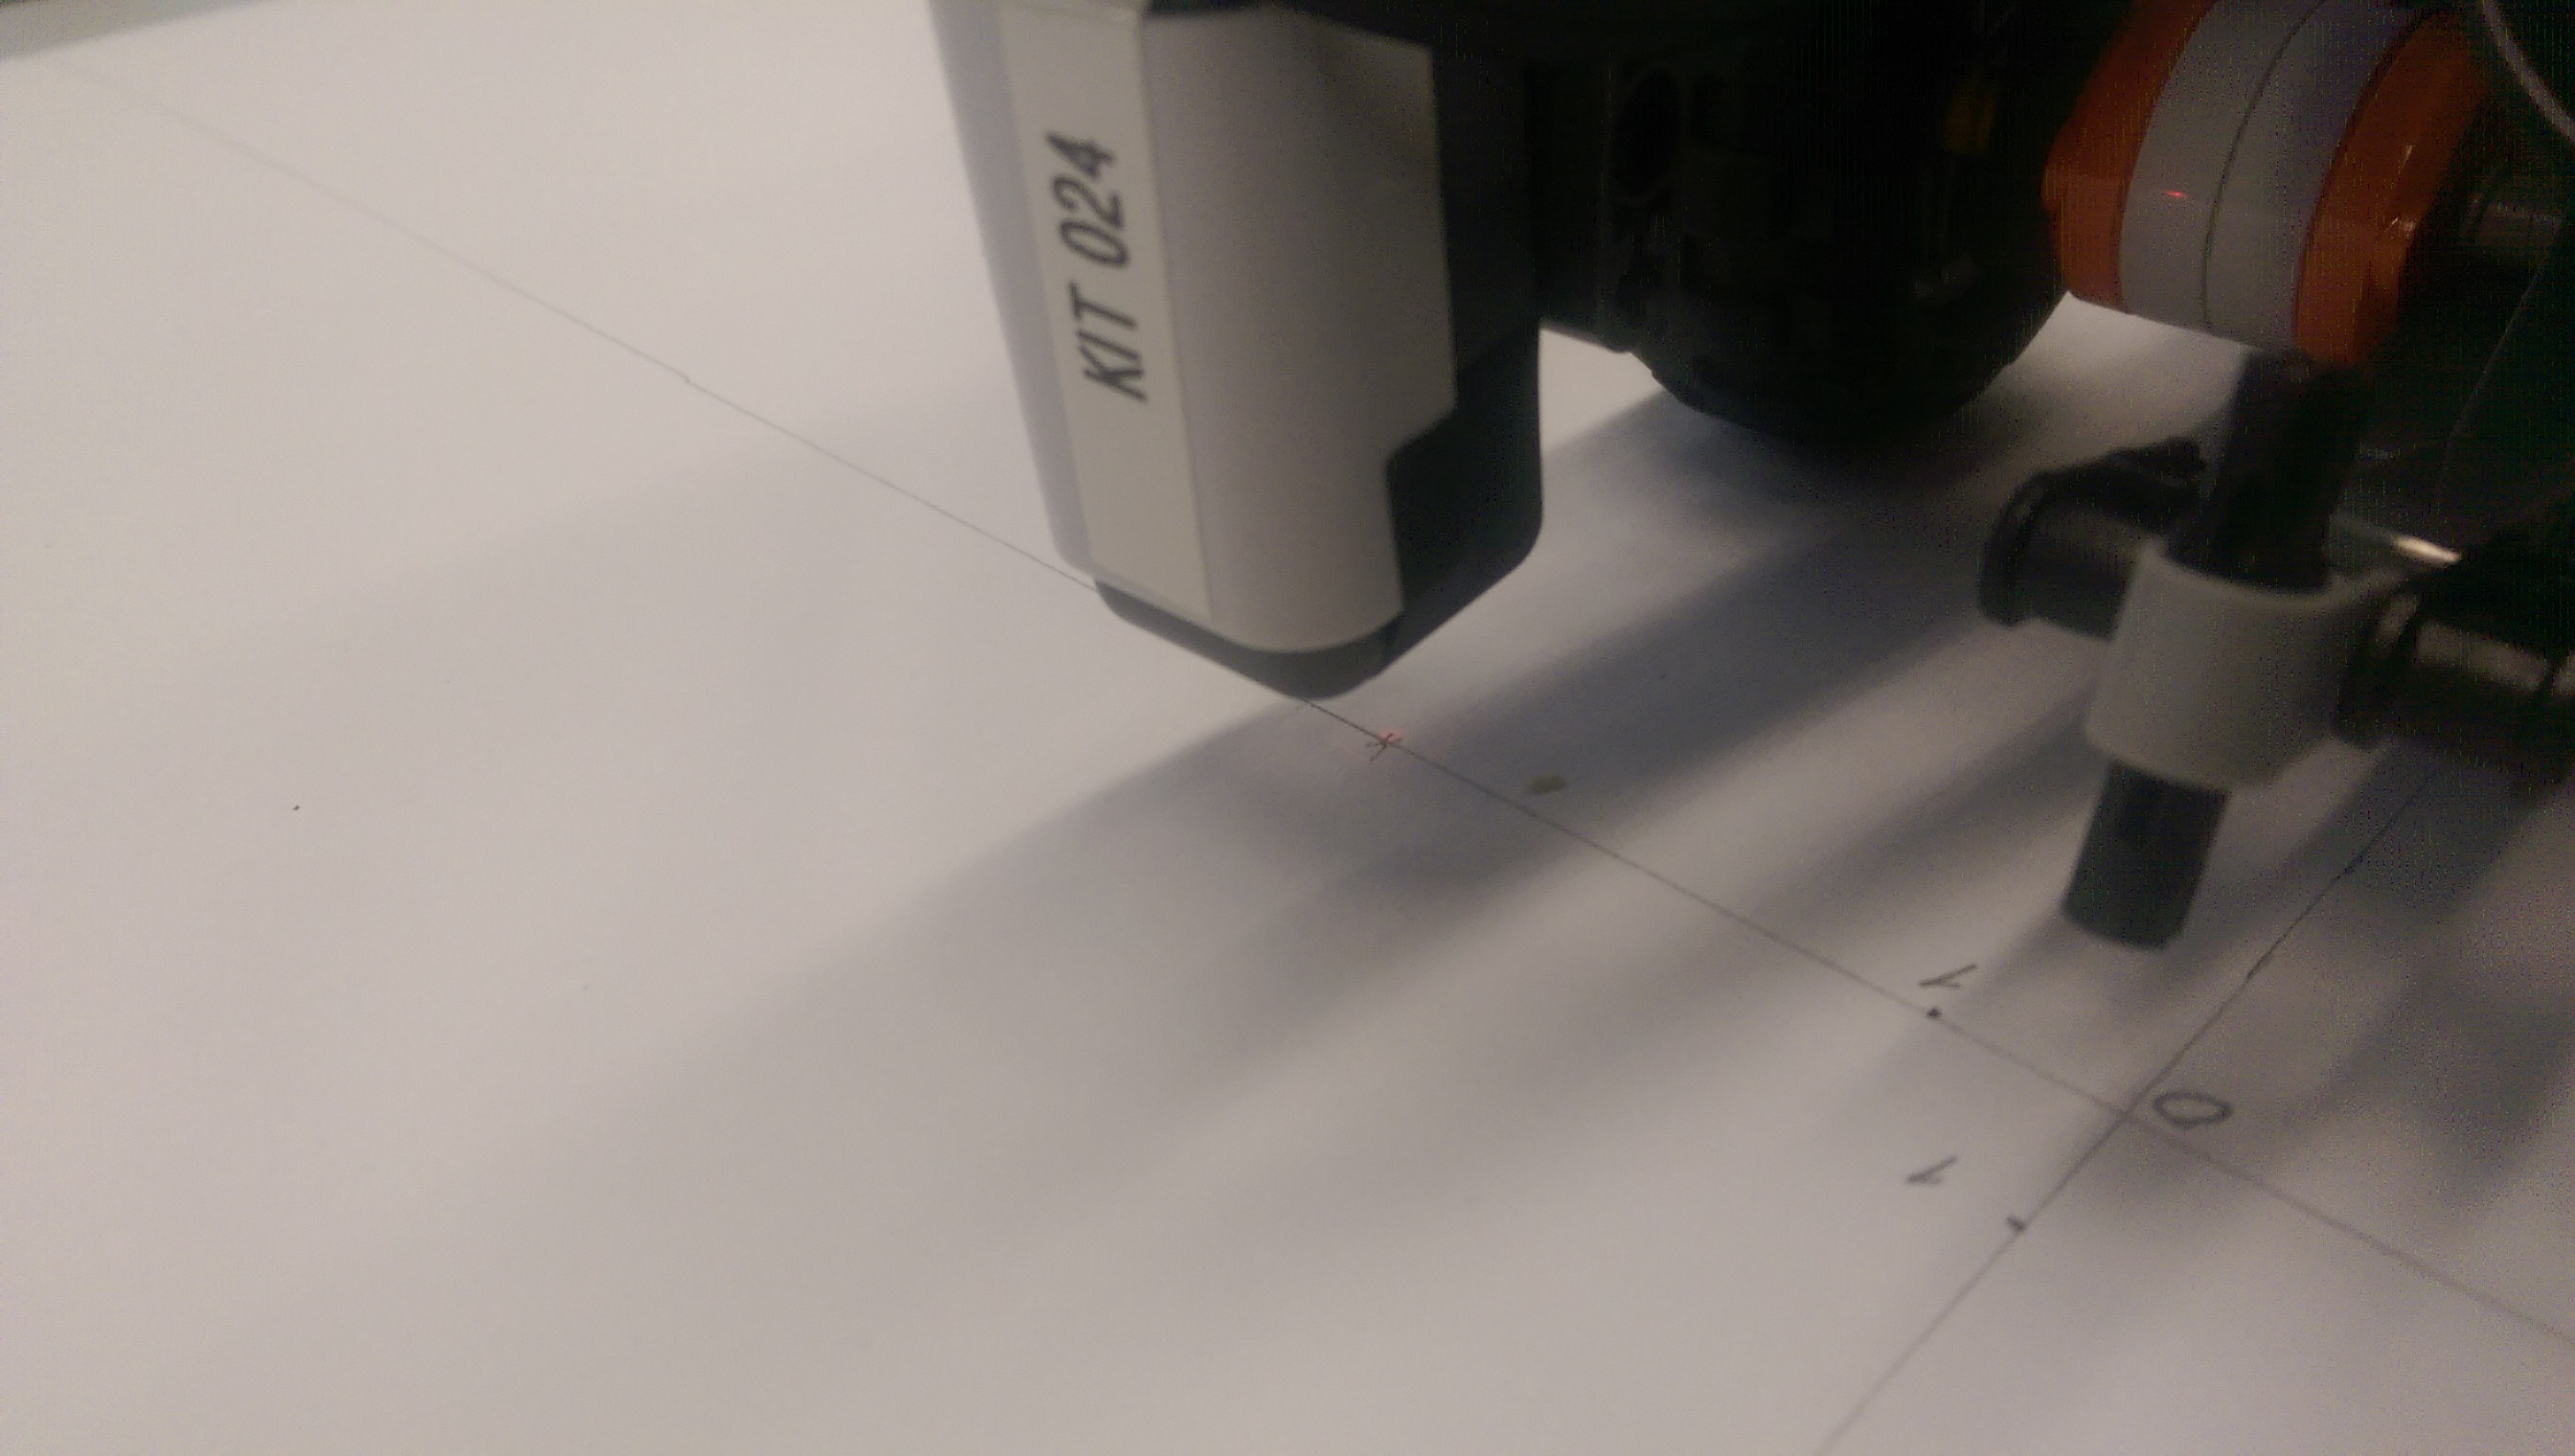
\includegraphics[width=1\linewidth]{images/IMAG0141}
            \caption{Right marker}
            \label{fig:img4}
        \end{minipage}
    \end{figure}

    \begin{figure}
        \centering
        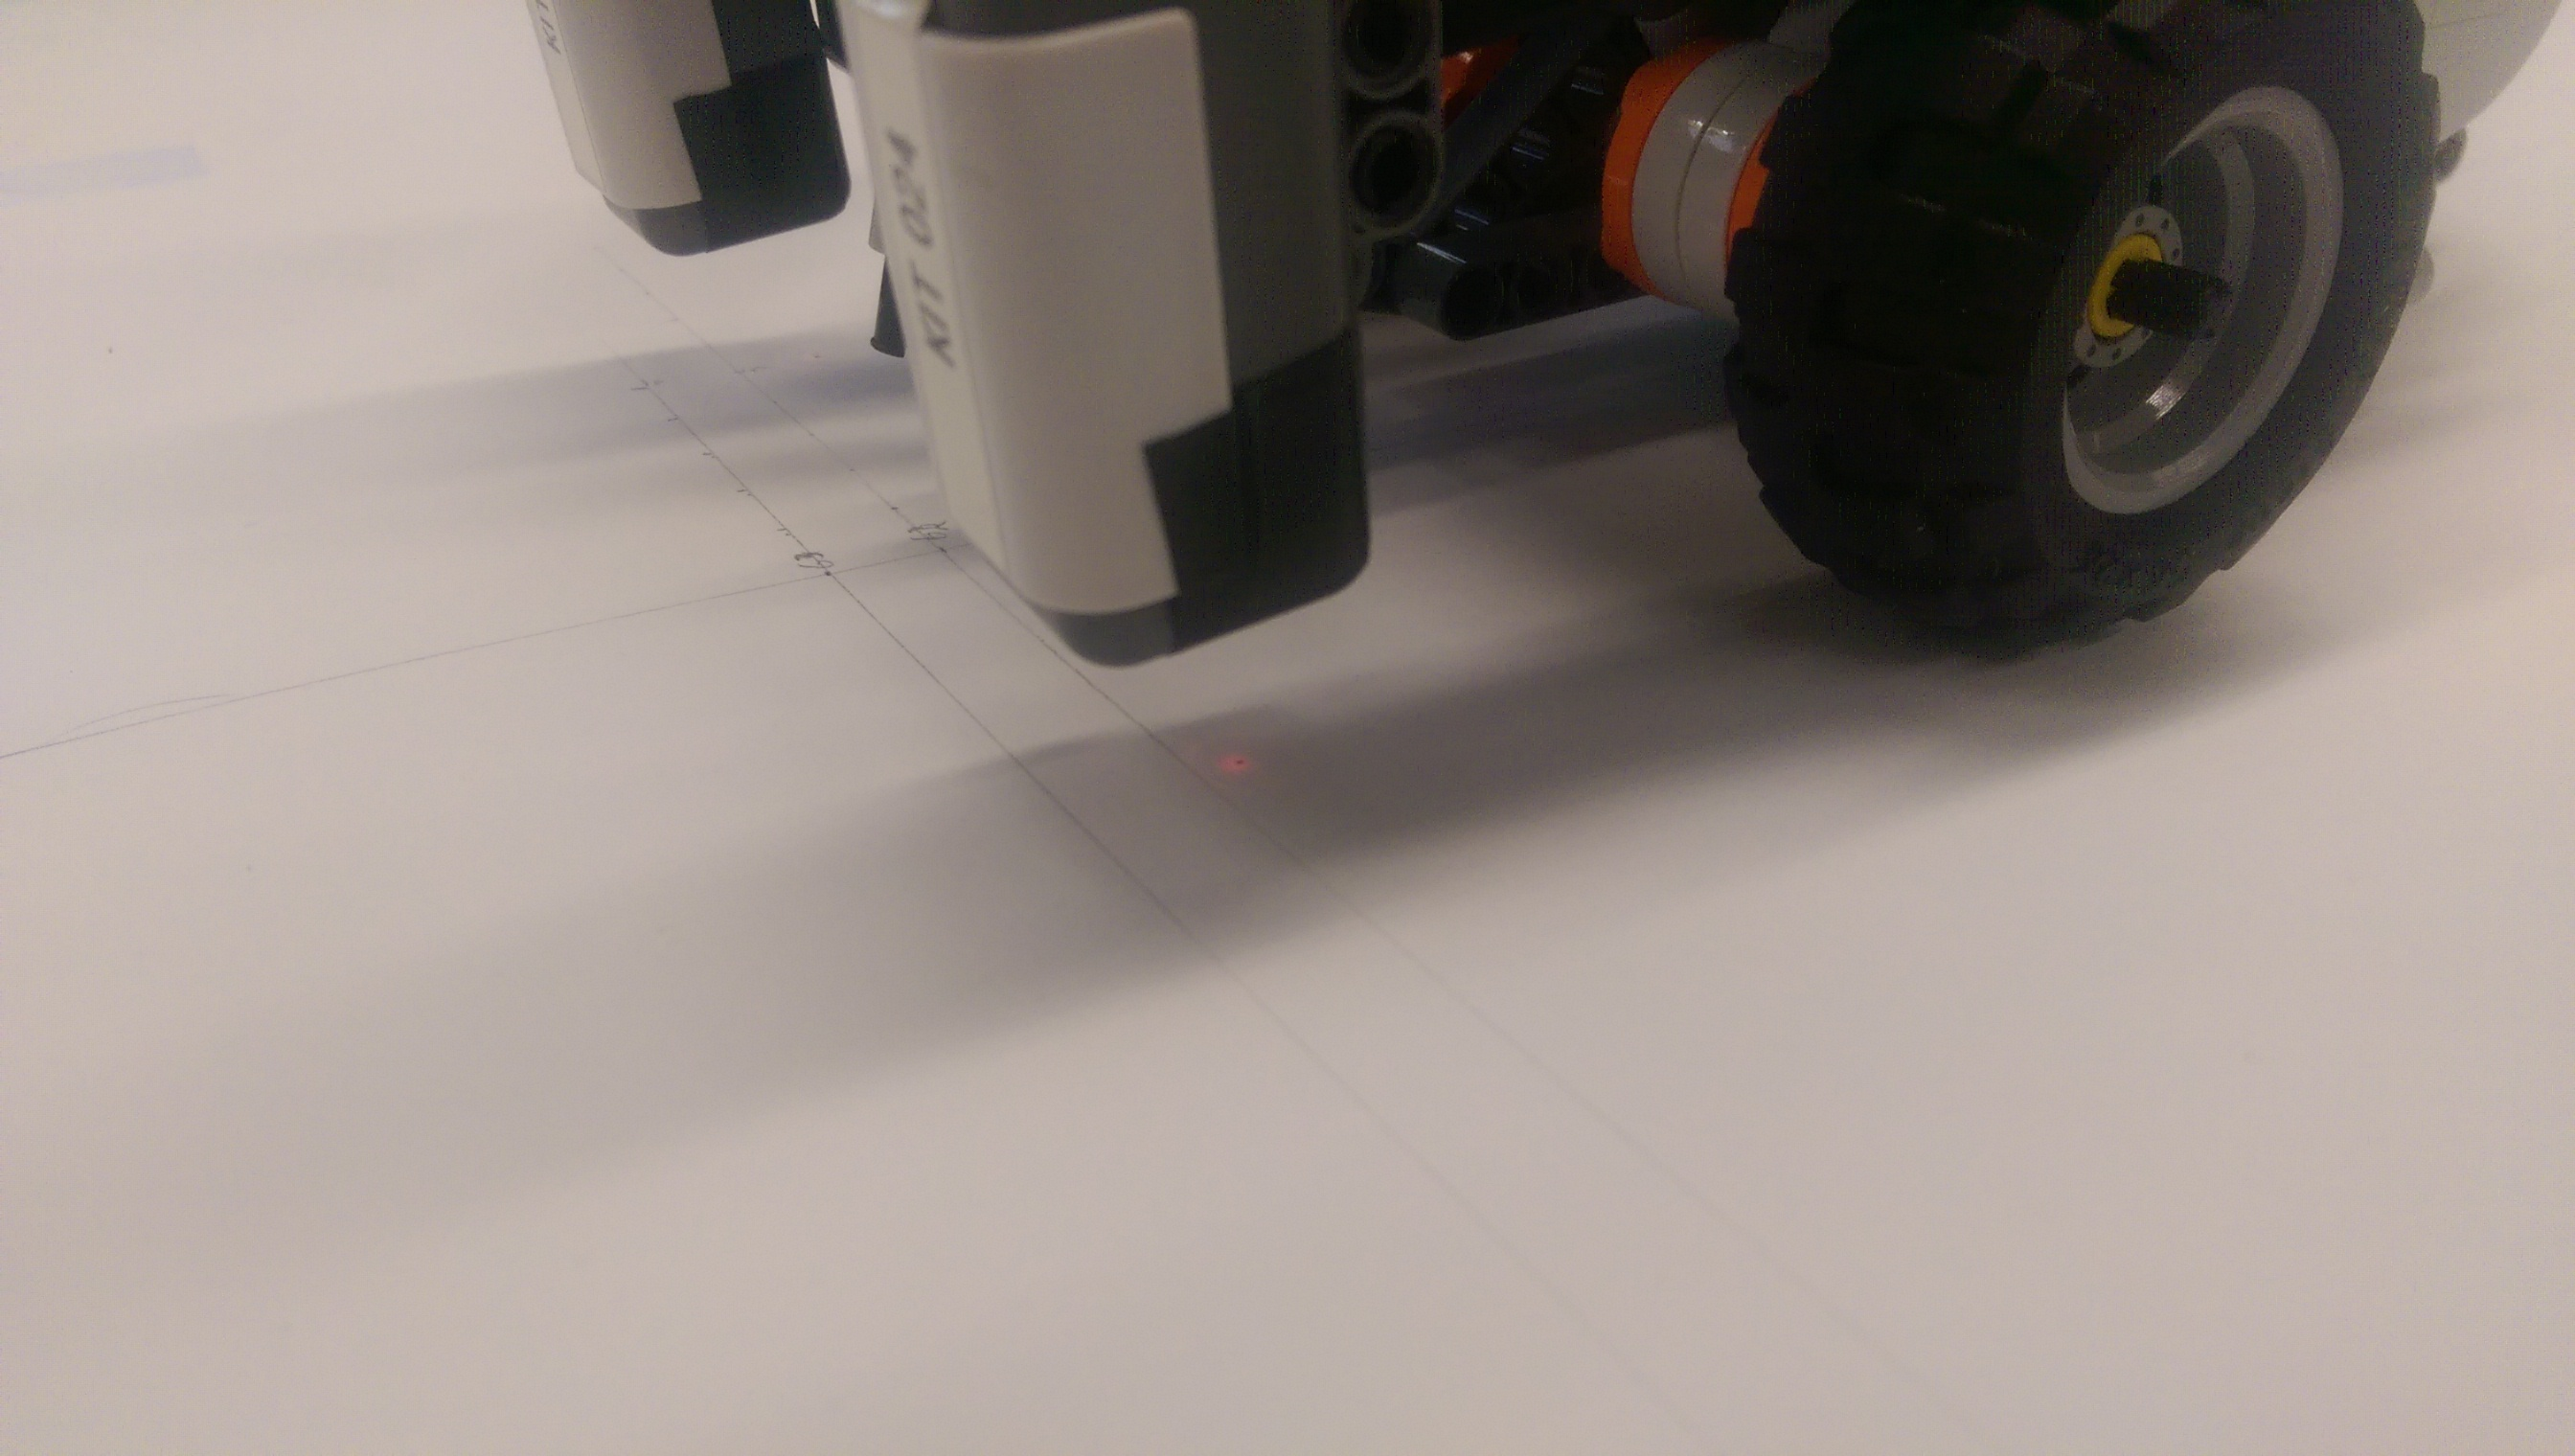
\includegraphics[width=0.9\linewidth]{images/IMAG0139}
        \caption{End point mark}
        \label{fig:img5}
    \end{figure}

    \begin{figure}[h!]
        \centering
        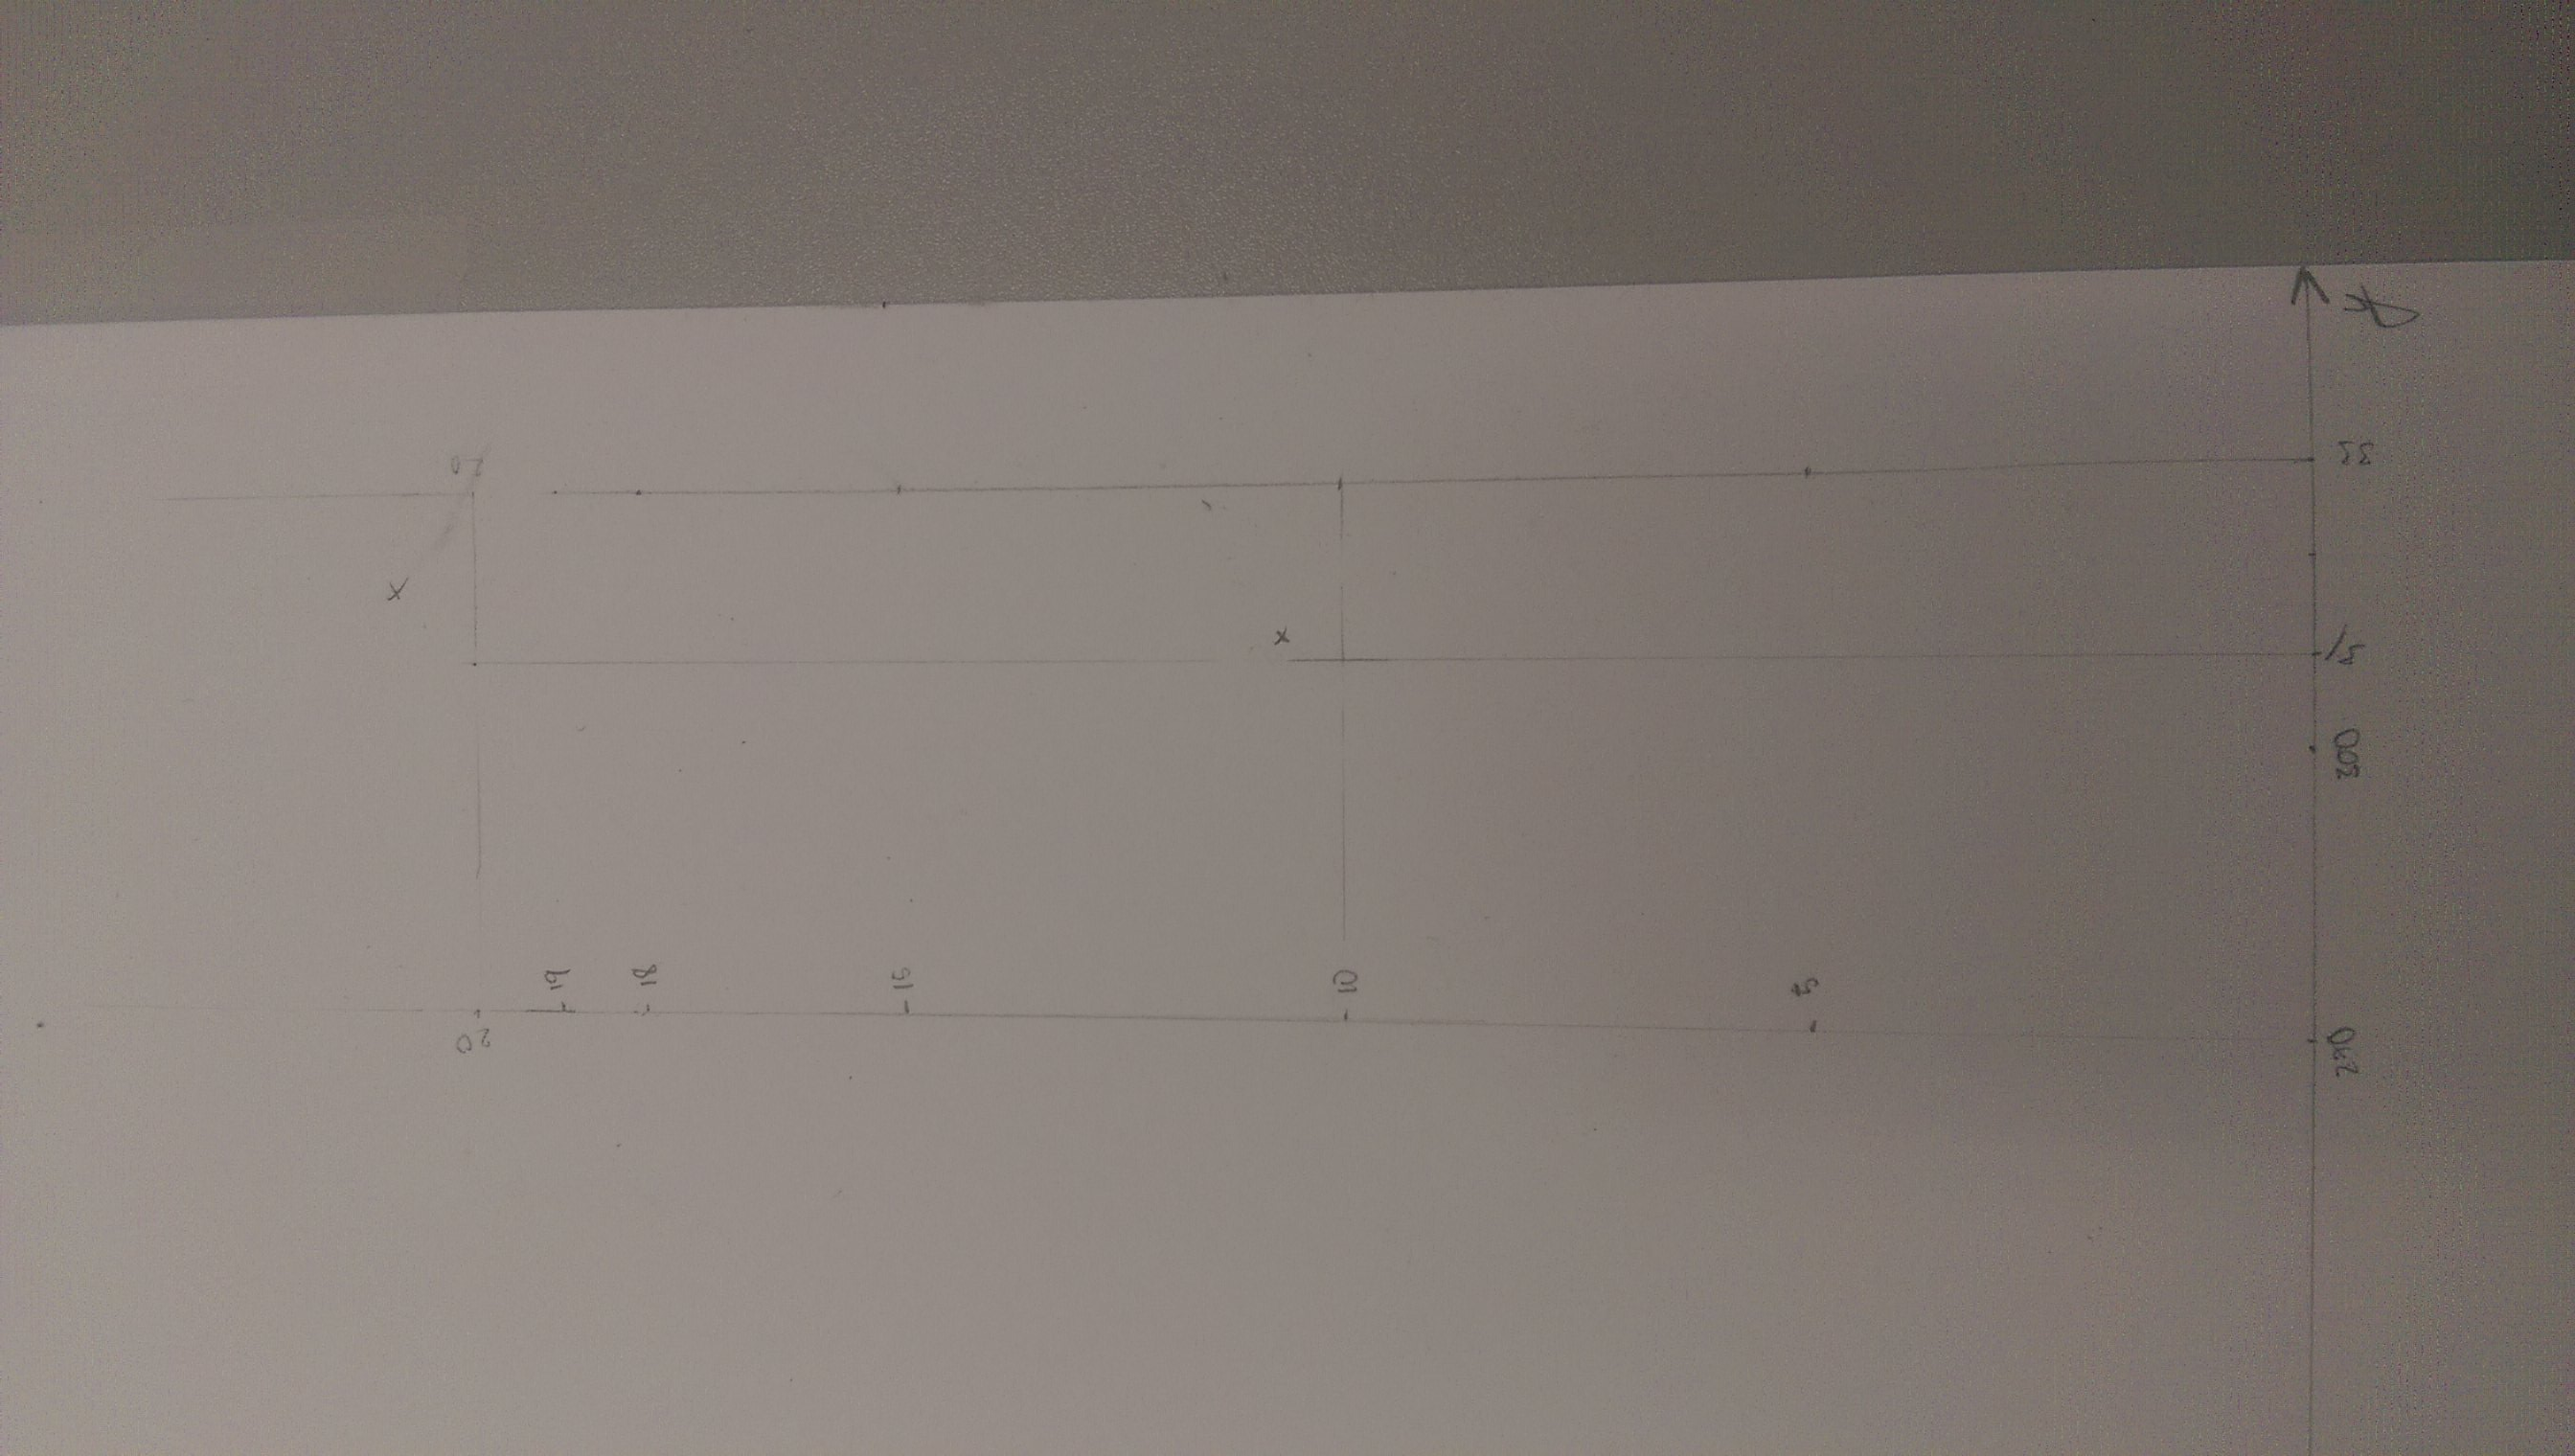
\includegraphics[width=0.9\linewidth]{images/IMAG0148}
        \caption{Mark measuring}
        \label{fig:img6}
    \end{figure}
    
    \subsection{Robot design}
    \begin{itemize}
        \item Wheels arrangement and light marker are the most important aspect of the robot design:
        \begin{itemize}
            \item The robot has two large front wheel and a small rear caster wheel.
            \item Two light markers are placed in the front, one on the left side and the other on the right side.
            \item These markers are placed closed to the ground.
            \item The light markers are also covered with tape, which have a small hole, to make the light mark on the ground similar to a point.
            \item The placement of the light markers is done so that the two point marks on the ground make a line, which is parallel to the wheel axle and its middle point is on the center line of the robot.
        \end{itemize}
    \end{itemize}

    \pagebreak
    \subsection{Measurement process}
    \begin{itemize}
        \item Before the measurements, we taped the white paper sheet onto a flat table surface. We make sure that the paper is as flat as possible.
        \item A x,y-coordinate system and a start point (figure \ref{fig:img2}) is drawn on the paper.
        \item Measurement for each experiment is done as follow:
        \begin{enumerate}
            \item Robot is initiated and placed onto the start point (figure \ref{fig:img2}). The two light marks should be on pre-marked points (figure \ref{fig:img3}, \ref{fig:img4}). The rear caster wheel's axle must be perpendicular to the robot's heading direction.
            \item Robot is started with as little force as possible. We make sure not to touch the robot while it is moving.
            \item After the robot stop, the two light marks on the paper is marked with pencil. We tried not to touch the robot while doing the marking (figure \ref{fig:img5}).
            \item The x,y-coordinate of two pencil marks is measured with rulers and is recorded (figure \ref{fig:img6}).
            \item The robot is then placed back onto the starting position for the next experiment.
        \end{enumerate}
    
    \end{itemize}

    \section{Experiment results}

    \begin{figure}[h!]
        \begin{center}
            \setlength{\fboxsep}{0.5pt} %
            \setlength{\fboxrule}{0.5pt}
            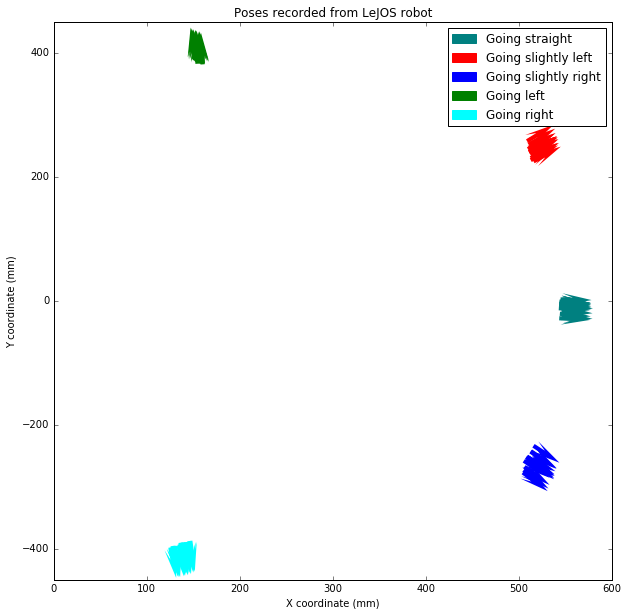
\includegraphics[width=14cm,fbox]{images/poses_plot_5_experiments.png}
            \caption{Recorded poses of the LeJOS robot executing five different motions.}
        \end{center}
    \end{figure}

    \newpage
    \subsection{Going straight forward}
    \begin{figure}[h!]
        \begin{center}
            \setlength{\fboxsep}{0.5pt} %
            \setlength{\fboxrule}{0.5pt}
            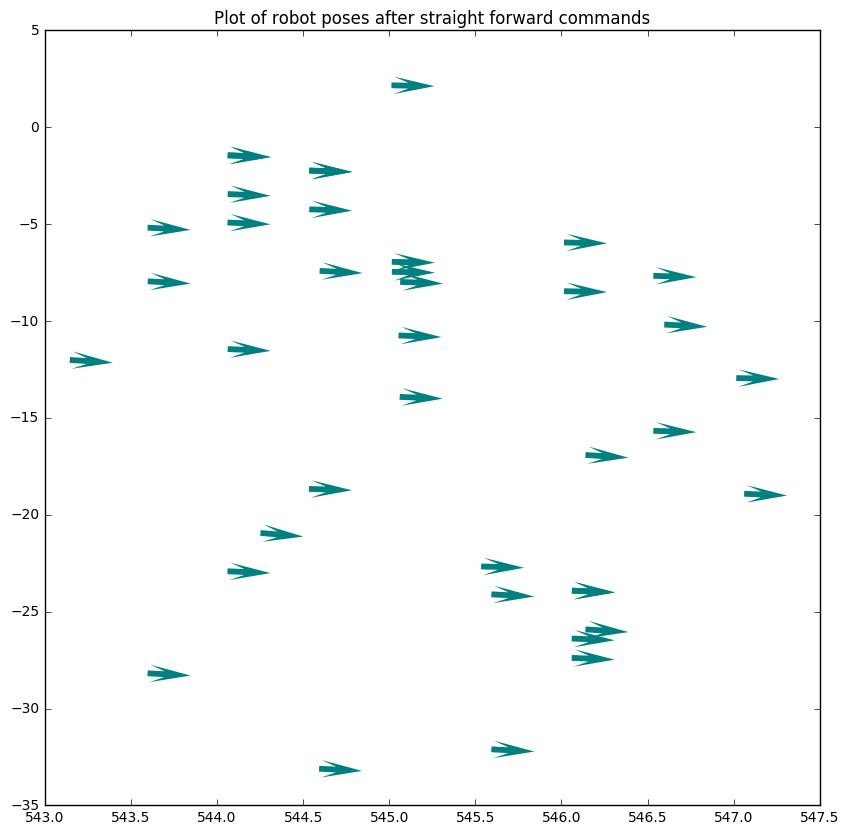
\includegraphics[width=10cm,fbox]{images/poses_plot_1_straight.png}
            \caption{Recorded poses of the LeJOS robot going straight forward.}
        \end{center}
    \end{figure}
    \begin{figure}[h!]
        \centering
        \begin{subfigure}[b]{0.3\textwidth}
            \setlength{\fboxsep}{0.5pt} %
            \setlength{\fboxrule}{0.5pt}
            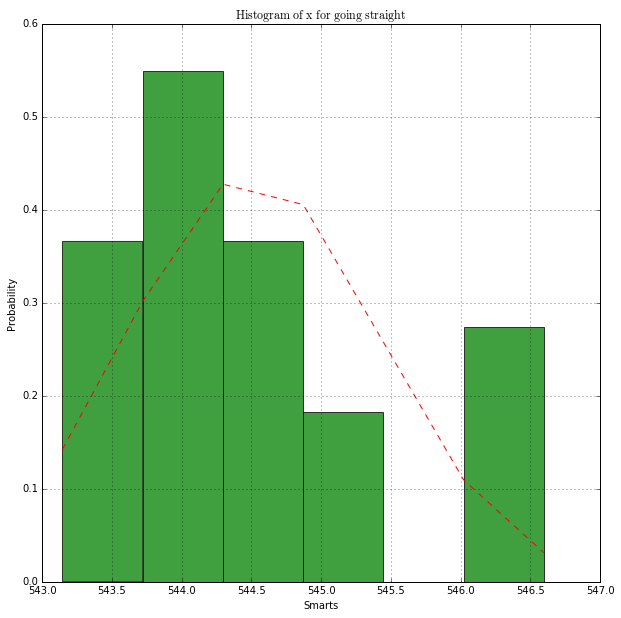
\includegraphics[width=\textwidth,fbox]{images/histogram_1_x_straight.png}
            \caption{$x$, $\mu = 544.508$, $\sigma = 0.908$}
        \end{subfigure}
        ~
        \begin{subfigure}[b]{0.3\textwidth}
            \setlength{\fboxsep}{0.5pt} %
            \setlength{\fboxrule}{0.5pt}
            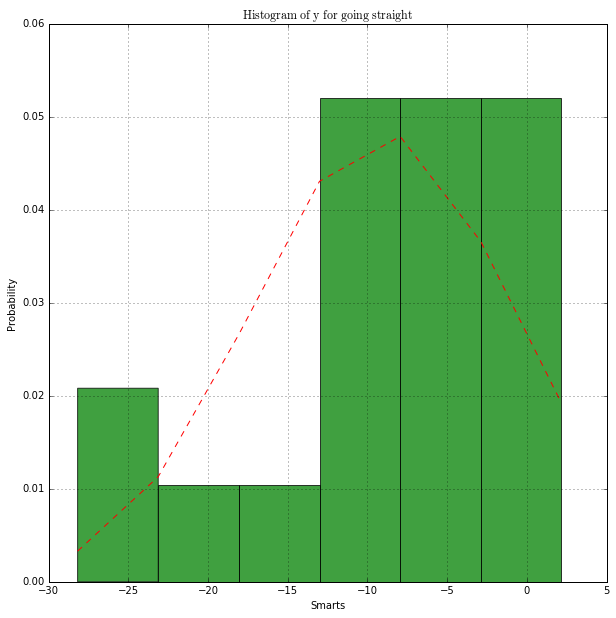
\includegraphics[width=\textwidth,fbox]{images/histogram_1_y_straight.png}
            \caption{$y$, $\mu = -9.045$, $\sigma = 8.257$}
        \end{subfigure}
        ~
        \begin{subfigure}[b]{0.3\textwidth}
            \setlength{\fboxsep}{0.5pt} %
            \setlength{\fboxrule}{0.5pt}
            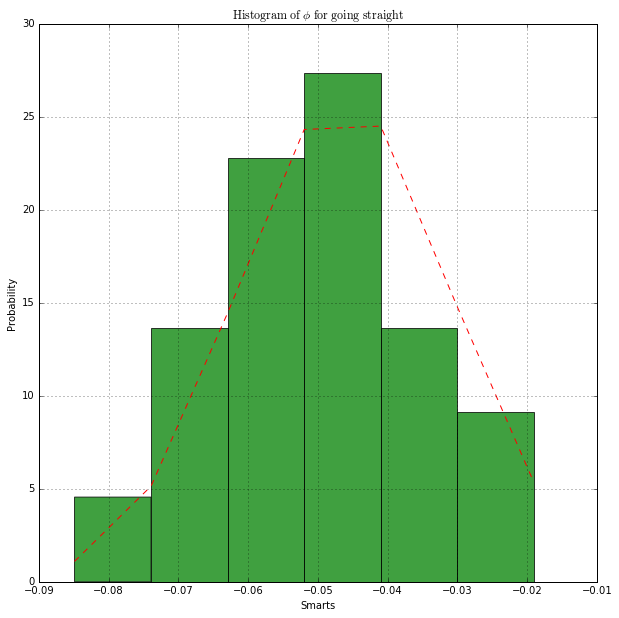
\includegraphics[width=\textwidth,fbox]{images/histogram_1_phi_straight.png}
            \caption{$\phi$, $\mu = -0.048$, $\sigma = 0.015$}
        \end{subfigure}
        \caption{Histograms of recorded coordinates and heading after straight movement}
    \end{figure}
    
    \newpage
    \subsection{Going slightly left}
    \begin{figure}[h]
        \begin{center}
            \setlength{\fboxsep}{0.5pt} %
            \setlength{\fboxrule}{0.5pt}
            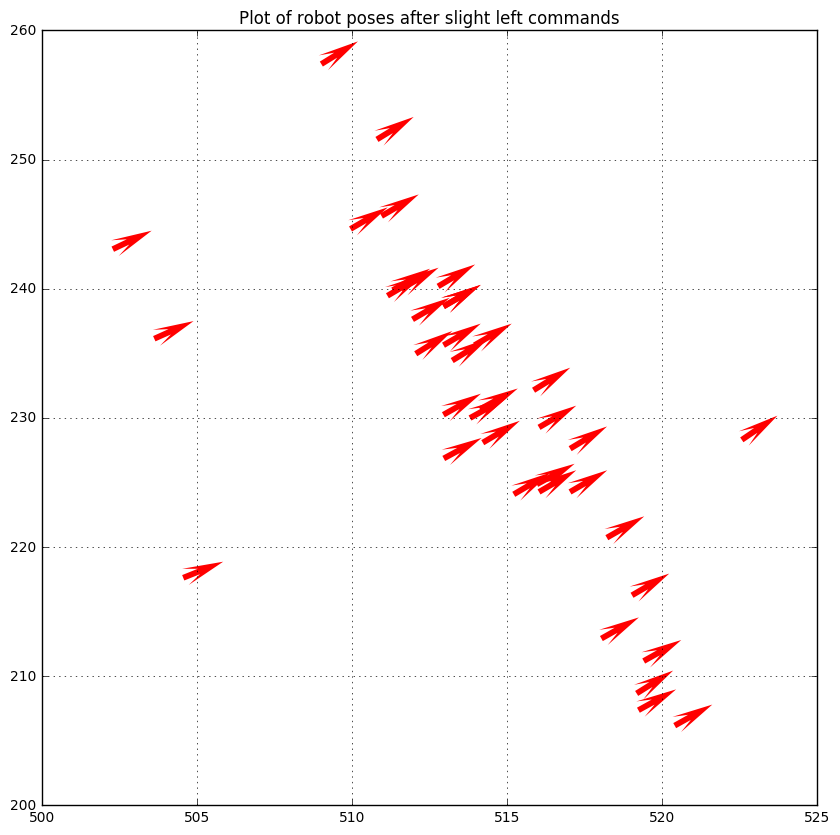
\includegraphics[width=10cm,fbox]{images/poses_plot_2_slightLeft.png}
            \caption{Recorded poses of the LeJOS robot going slightly left.}
        \end{center}
    \end{figure}
    \begin{figure}[h!]
        \centering
        \begin{subfigure}[b]{0.3\textwidth}
            \setlength{\fboxsep}{0.5pt} %
            \setlength{\fboxrule}{0.5pt}
            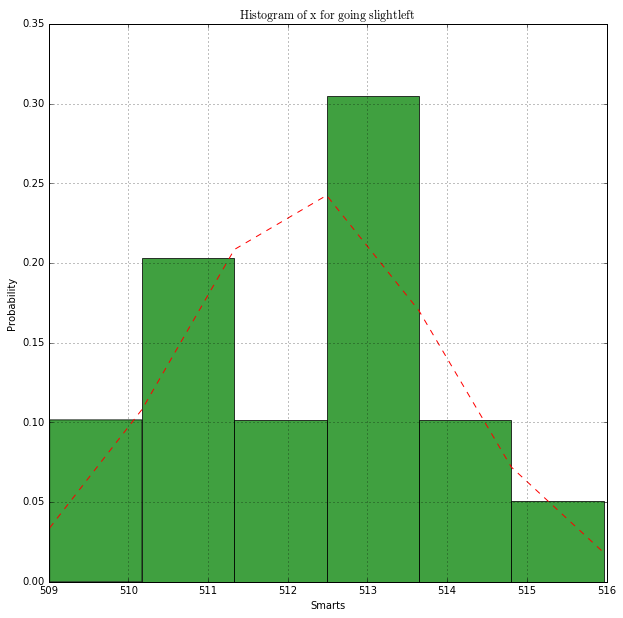
\includegraphics[width=\textwidth,fbox]{images/histogram_2_x_slightLeft.png}
            \caption{$x$, $\mu = 512.255$, $\sigma = 1.629$}
        \end{subfigure}
        ~
        \begin{subfigure}[b]{0.3\textwidth}
            \setlength{\fboxsep}{0.5pt} %
            \setlength{\fboxrule}{0.5pt}
            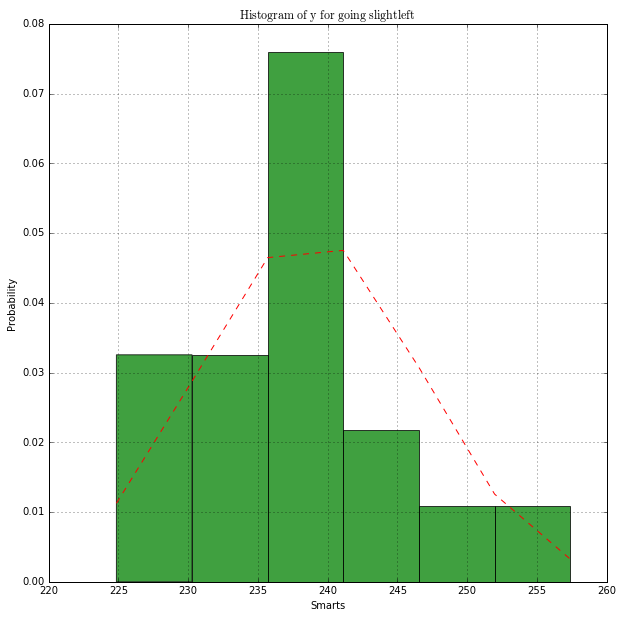
\includegraphics[width=\textwidth,fbox]{images/histogram_2_y_slightLeft.png}
            \caption{$y$, $\mu = 238.680$, $\sigma = 8.013$}
        \end{subfigure}
        ~
        \begin{subfigure}[b]{0.3\textwidth}
            \setlength{\fboxsep}{0.5pt} %
            \setlength{\fboxrule}{0.5pt}
            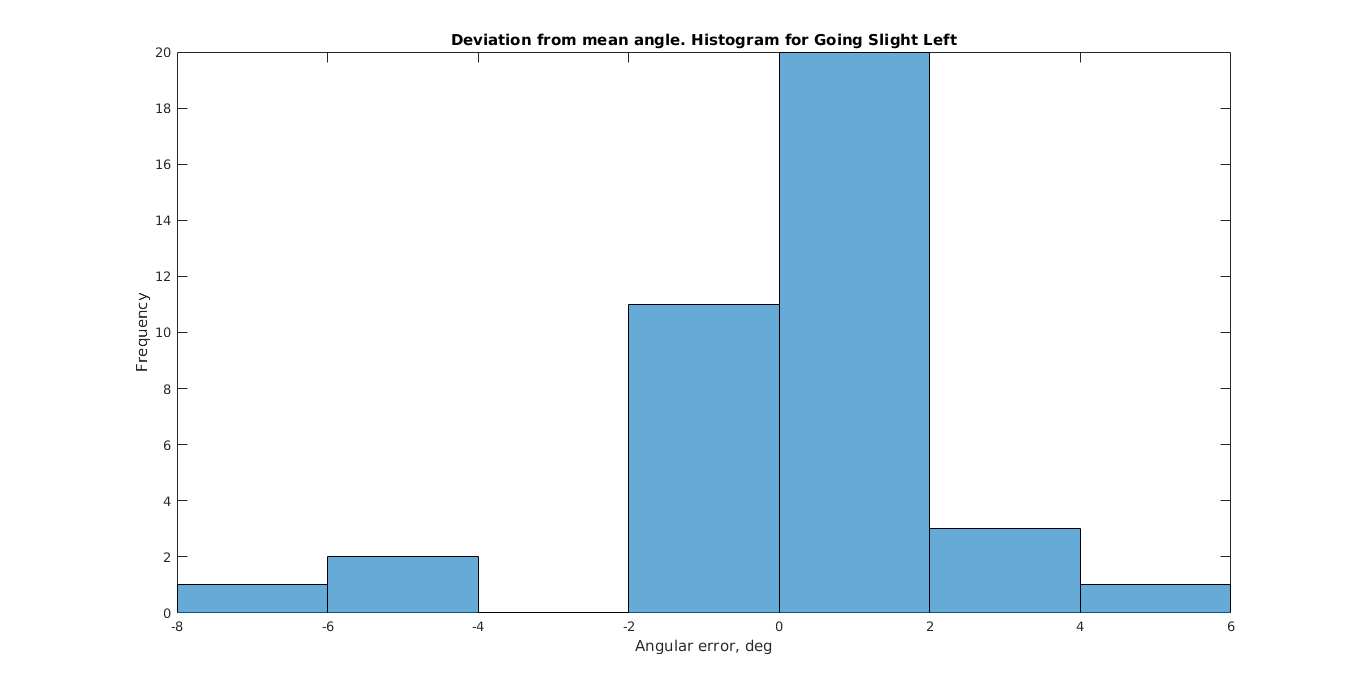
\includegraphics[width=\textwidth,fbox]{images/histogram_2_phi_slightLeft.png}
            \caption{$\phi$, $\mu = 0.523$, $\sigma = 0.015$}
        \end{subfigure}
        \caption{Histograms of recorded coordinates and heading after a slightly left movement}
    \end{figure}

    \newpage
    \subsection{Going slightly right}
    \begin{figure}[h!]
        \begin{center}
            \setlength{\fboxsep}{0.5pt} %
            \setlength{\fboxrule}{0.5pt}
            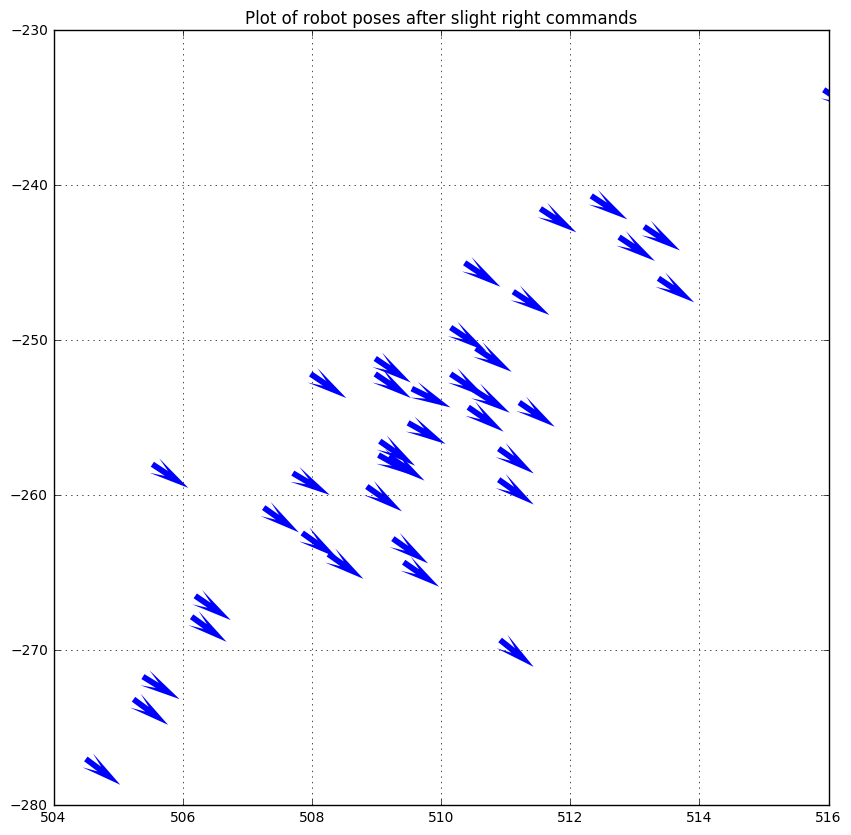
\includegraphics[width=12cm,fbox]{images/poses_plot_3_slightRight.png}
            \caption{Recorded poses of the LeJOS robot going slightly right.}
        \end{center}
    \end{figure}
    \begin{figure}[h!]
        \centering
        \begin{subfigure}[b]{0.3\textwidth}
            \setlength{\fboxsep}{0.5pt} %
            \setlength{\fboxrule}{0.5pt}
            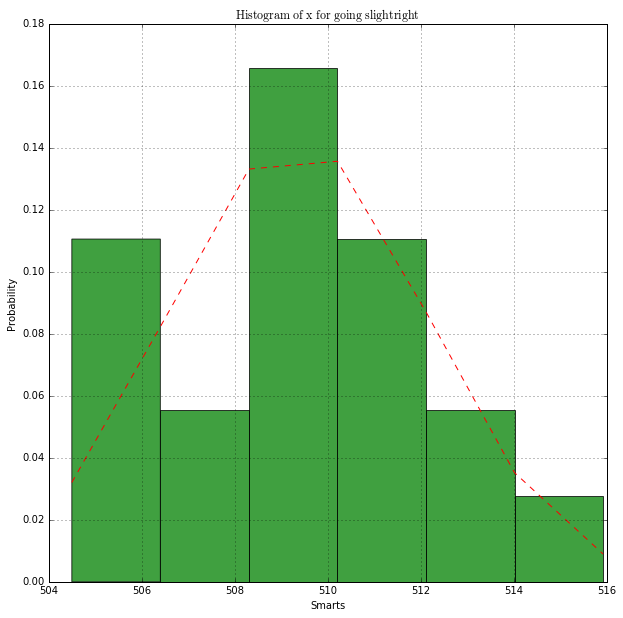
\includegraphics[width=\textwidth,fbox]{images/histogram_3_x_slightRight.png}
            \caption{$x$, $\mu = 509.338$, $\sigma = 2.801$}
        \end{subfigure}
        ~
        \begin{subfigure}[b]{0.3\textwidth}
            \setlength{\fboxsep}{0.5pt} %
            \setlength{\fboxrule}{0.5pt}
            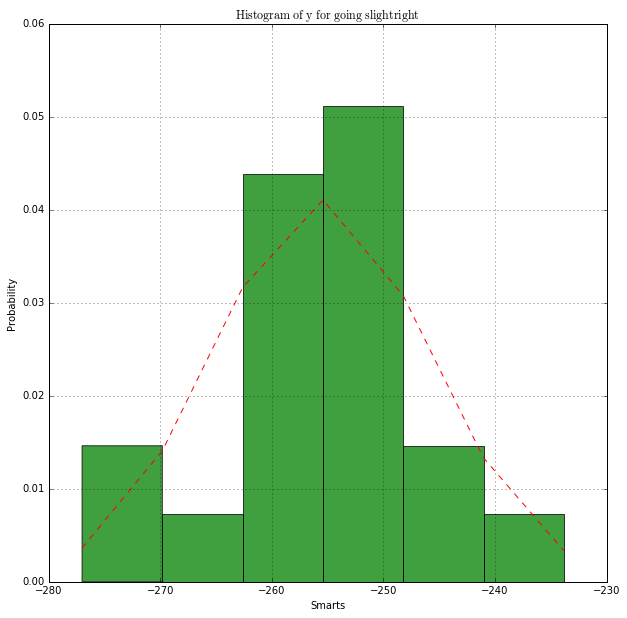
\includegraphics[width=\textwidth,fbox]{images/histogram_3_y_slightRight.png}
            \caption{$y$, $\mu = -255.601$, $\sigma = 9.714$}
        \end{subfigure}
        ~
        \begin{subfigure}[b]{0.3\textwidth}
            \setlength{\fboxsep}{0.5pt} %
            \setlength{\fboxrule}{0.5pt}
            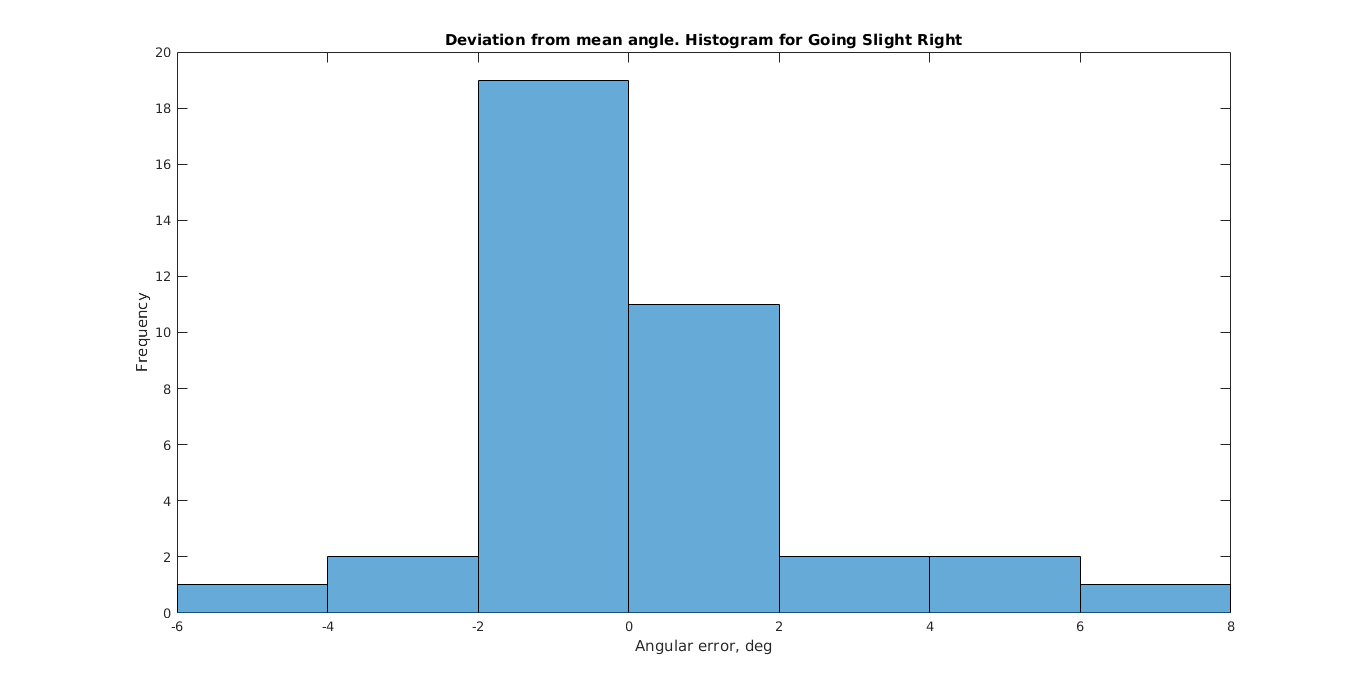
\includegraphics[width=\textwidth,fbox]{images/histogram_3_phi_slightRight.png}
            \caption{$\phi$, $\mu = -0.583$, $\sigma = 0.047$}
        \end{subfigure}
        \caption{Histograms of recorded coordinates and heading after a slightly right movement}
    \end{figure}

\newpage
\subsection{Going left}
\begin{figure}[h!]
    \begin{center}
        \setlength{\fboxsep}{0.5pt} %
        \setlength{\fboxrule}{0.5pt}
        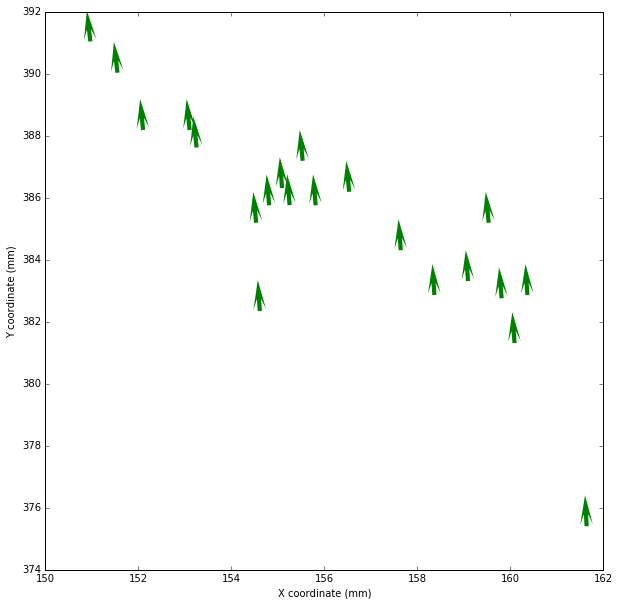
\includegraphics[width=12cm,fbox]{images/poses_plot_4_left.png}
        \caption{Recorded poses of the LeJOS robot going left.}
    \end{center}
\end{figure}
\begin{figure}[h!]
    \centering
    \begin{subfigure}[b]{0.3\textwidth}
        \setlength{\fboxsep}{0.5pt} %
        \setlength{\fboxrule}{0.5pt}
        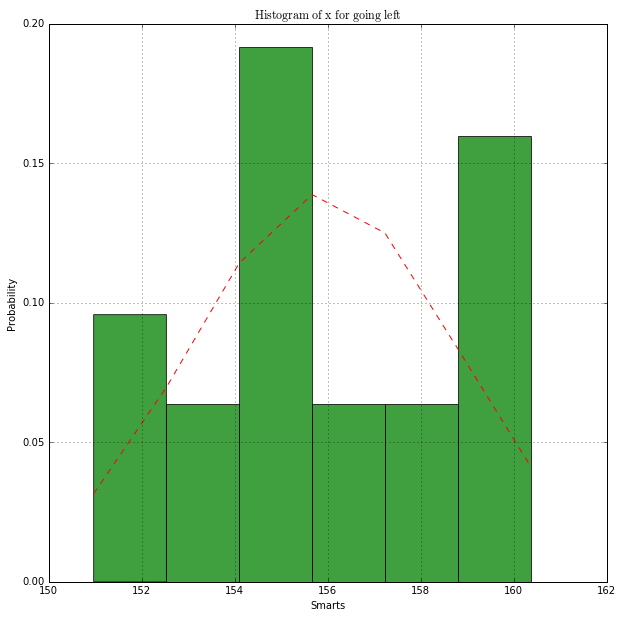
\includegraphics[width=\textwidth,fbox]{images/histogram_4_x_left.png}
        \caption{$x$, $\mu = 155.903$, $\sigma = 2.865$}
    \end{subfigure}
    ~
    \begin{subfigure}[b]{0.3\textwidth}
        \setlength{\fboxsep}{0.5pt} %
        \setlength{\fboxrule}{0.5pt}
        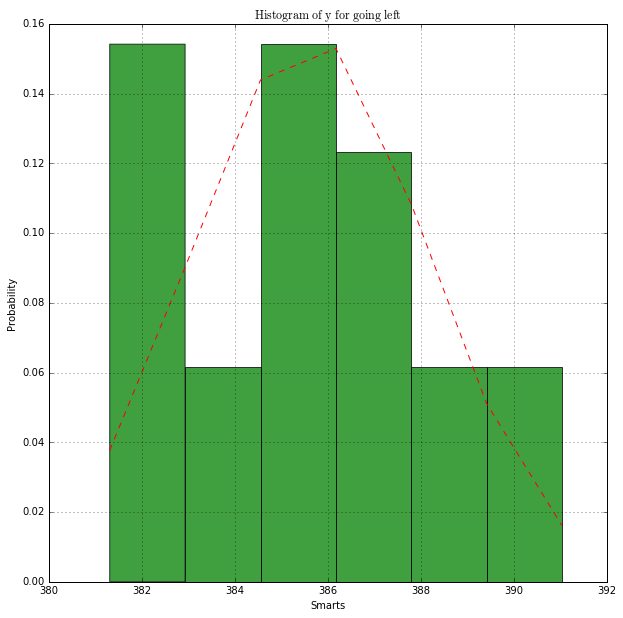
\includegraphics[width=\textwidth,fbox]{images/histogram_4_y_left.png}
        \caption{$y$, $\mu = 385.611$, $\sigma = 2.545$}
    \end{subfigure}
    ~
    \begin{subfigure}[b]{0.3\textwidth}
        \setlength{\fboxsep}{0.5pt} %
        \setlength{\fboxrule}{0.5pt}
        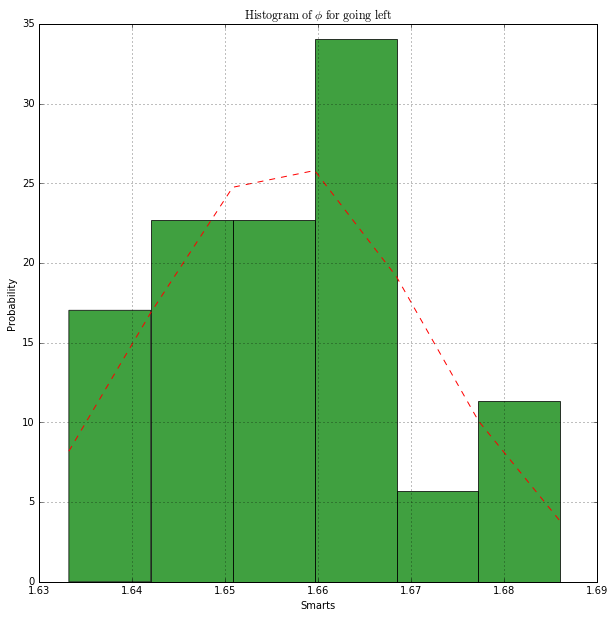
\includegraphics[width=\textwidth,fbox]{images/histogram_4_phi_left.png}
        \caption{$\phi$, $\mu = 1.656$, $\sigma = 0.0151$}
    \end{subfigure}
    \caption{Histograms of recorded coordinates and heading after a left movement.}
\end{figure}

\newpage
\subsection{Going right}
\begin{figure}[h!]
    \begin{center}
        \setlength{\fboxsep}{0.5pt} %
        \setlength{\fboxrule}{0.5pt}
        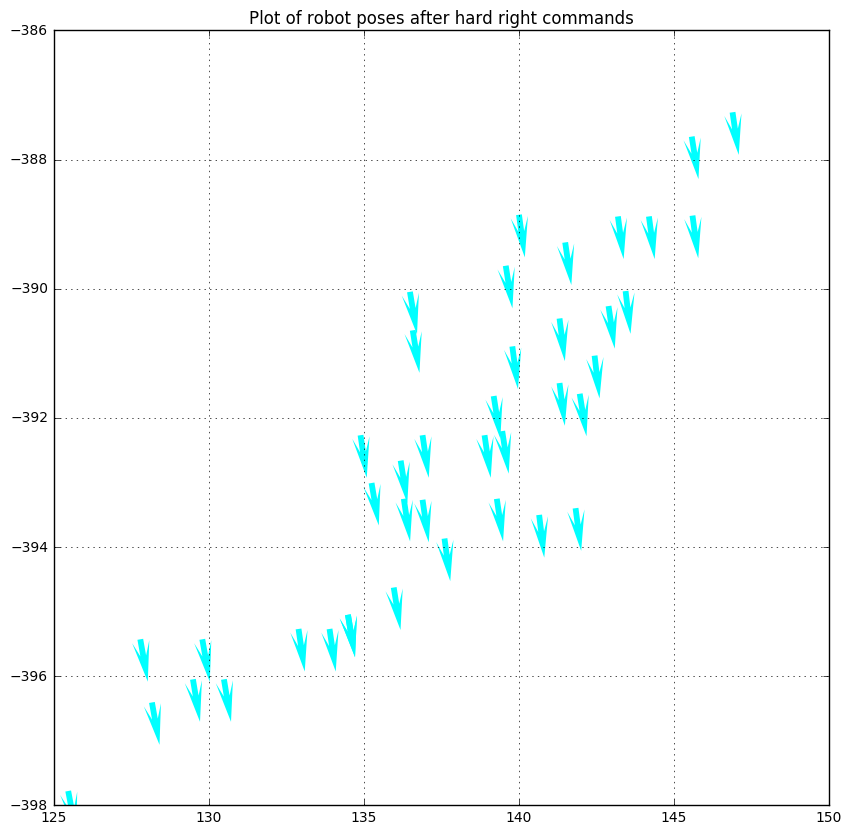
\includegraphics[width=12cm,fbox]{images/poses_plot_5_right.png}
        \caption{Recorded poses of the LeJOS robot going right.}
    \end{center}
\end{figure}
\begin{figure}[h!]
    \centering
    \begin{subfigure}[b]{0.3\textwidth}
        \setlength{\fboxsep}{0.5pt} %
        \setlength{\fboxrule}{0.5pt}
        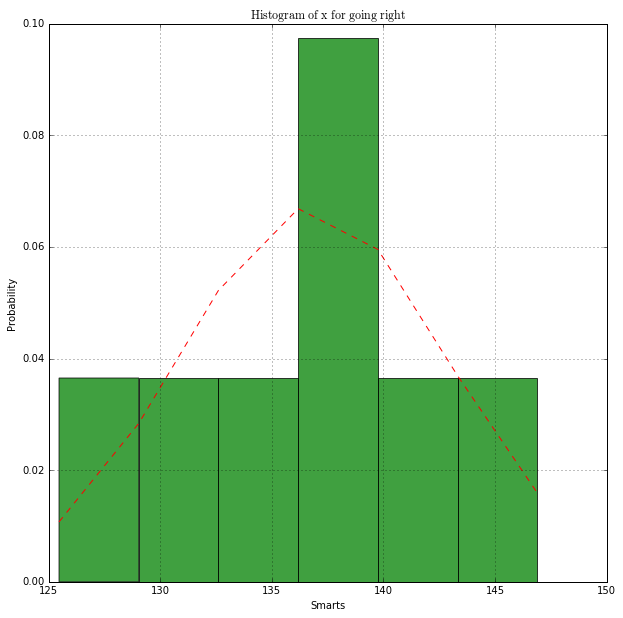
\includegraphics[width=\textwidth,fbox]{images/histogram_5_x_right.png}
        \caption{$x$, $\mu = 136.830$, $\sigma = 5.931$}
    \end{subfigure}
    ~
    \begin{subfigure}[b]{0.3\textwidth}
        \setlength{\fboxsep}{0.5pt} %
        \setlength{\fboxrule}{0.5pt}
        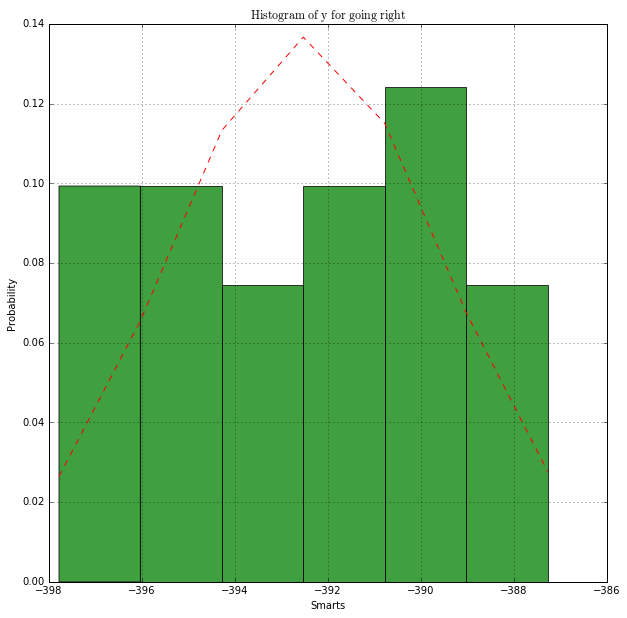
\includegraphics[width=\textwidth,fbox]{images/histogram_5_y_right.png}
        \caption{$y$, $\mu = -392.485$, $\sigma = 2.919$}
    \end{subfigure}
    ~
    \begin{subfigure}[b]{0.3\textwidth}
        \setlength{\fboxsep}{0.5pt} %
        \setlength{\fboxrule}{0.5pt}
        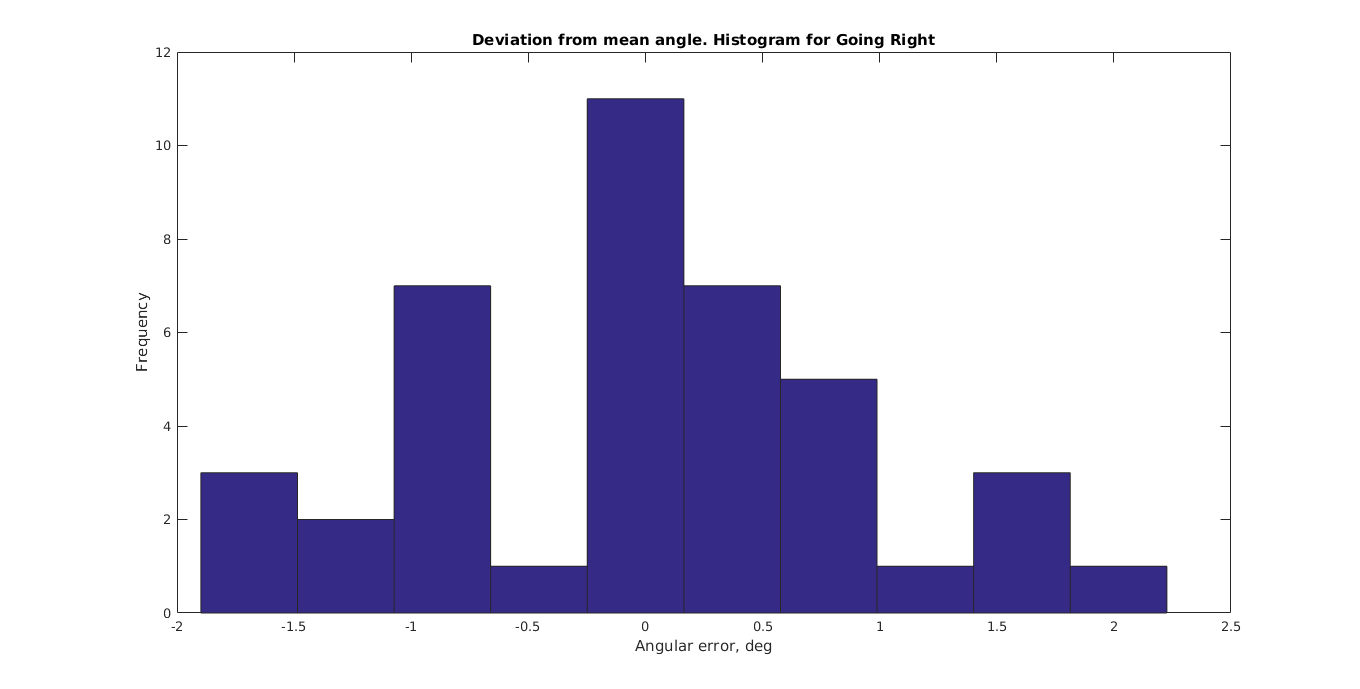
\includegraphics[width=\textwidth,fbox]{images/histogram_5_phi_right.png}
        \caption{$\phi$, $\mu = -1.412$, $\sigma = 0.013$}
    \end{subfigure}
    \caption{Histograms of recorded coordinates and heading after a right movement.}
\end{figure}

\newpage
\section{Conclusion}
From the data, it can be seen that the variation in the robot's heading direction is much smaller than the variantion in the direction perpendicular to the robot's heading direction.
This behaviour seems to be caused by the unsymmetrical property of two motors, wheels. Most of the graphs show a peak close to the center. They are not totally symmetrical and clearly guassian-like, but this can be fixed by taking more samples. An important note is that the battery level is very critical to the result of the experiment. Lower battery level can cause a constant shift in the experiment output.
\end{document}
